\documentclass[a4paper, 12pt, english]{article}

\usepackage[utf8]{inputenc}
\usepackage{amsmath,amssymb}
\usepackage{graphicx}
\usepackage{subfig}
\usepackage[colorinlistoftodos]{todonotes}

\usepackage{indentfirst}
\usepackage{verbatim}
\usepackage{textcomp}
\usepackage{gensymb}

\usepackage{relsize}

\usepackage{lipsum}% http://ctan.org/pkg/lipsum
\usepackage{xcolor}% http://ctan.org/pkg/xcolor
\usepackage{xparse}% http://ctan.org/pkg/xparse
\NewDocumentCommand{\myrule}{O{1pt} O{2pt} O{black}}{%
  \par\nobreak % don't break a page here
  \kern\the\prevdepth % don't take into account the depth of the preceding line
  \kern#2 % space before the rule
  {\color{#3}\hrule height #1 width\hsize} % the rule
  \kern#2 % space after the rule
  \nointerlineskip % no additional space after the rule
}
\usepackage[section]{placeins}

\usepackage{booktabs}
\usepackage{colortbl}%
   \newcommand{\myrowcolour}{\rowcolor[gray]{0.925}}
   
\usepackage[obeyspaces]{url}
\usepackage{etoolbox}
\usepackage[colorlinks,citecolor=black,urlcolor=blue,bookmarks=false,hypertexnames=true]{hyperref} 

\usepackage{geometry}
\geometry{
	paper=a4paper, % Change to letterpaper for US letter
	inner=1cm, % Inner margin
	outer=1cm, % Outer margin
	bindingoffset=.5cm, % Binding offset
	top=2cm, % Top margin
	bottom=2cm, % Bottom margin
	%showframe, % Uncomment to show how the type block is set on the page
}

\usepackage{float}

\usepackage{amsmath,amsfonts}

\usepackage{textcomp}

\usepackage{listings}
\DeclareCaptionFormat{listing}{\centerline#3}
\captionsetup[lstlisting]{format=listing,labelsep=none,justification=justified}

% MATLAB code formatting
\lstdefinestyle{matlab}{
    language=Matlab,
    basicstyle=\footnotesize\ttfamily,
    keywordstyle=\color{blue},
    commentstyle=\color{green!40!black},
    stringstyle=\color{red},
    showstringspaces=false,
    numbers=left,
    numberstyle=\footnotesize,
    numbersep=10pt,
    tabsize=2,
    breaklines=true,
    breakatwhitespace=true,
    captionpos=b
}

% MATLAB command window formatting
\lstdefinestyle{commandstyle}{
    basicstyle=\scriptsize\ttfamily,
    numbers=none,
    showstringspaces=false,
    breaklines=true,
    frame=single,
    frameround=fttt,
    backgroundcolor=\color{gray!10},
    xleftmargin=0.5cm,
    xrightmargin=0.5cm,
    captionpos=b
}
\usepackage{multicol,caption,subcaption}
\newenvironment{Figure}
  {\par\medskip\noindent\minipage{\linewidth}}
  {\endminipage\par\medskip}
\usepackage{array}

\newcommand{\highlight}[1]{\textcolor{blue}{\texttt{#1}}}

\graphicspath{{images/}}
\setlength {\marginparwidth }{2cm}

%*******************************************************************************%
%************************************START**************************************%
%*******************************************************************************%
\begin{document}

%************************************TITLE PAGE**************************************%
\begin{titlepage}
\begin{center}
\textbf{\LARGE Alexandria University}\\[0.5cm] 
\textbf{\large FACULTY OF ENGINEERING}\\[0.2cm]
\vspace{20pt}

\includegraphics{logo.png}\\[1cm]
\par
\vspace{20pt}
\textbf{\Large EEC-461 Antenna Engineering}\\
\vspace{15pt}
\myrule[1pt][7pt]
\textbf{\LARGE  LABORATORY REPORT 1}\\
\vspace{15pt}
\textbf{\large Analysis and Visualization of Antenna Radiation Patterns}\\
\myrule[1pt][7pt]
\vspace{25pt}
\textbf{\large \hspace{50pt}Student Name \hspace{60pt} Student ID}\\
Ahmed Osama Mohamed Afifi \hspace{60pt} 20010038 \\

\vspace{45pt}
%\textbf {\large Lecturer in charge:}\\[0.2cm]
%\Large {Ir. Chan Cheong Loong}\\[0.1cm]
\end{center}

\par
\vfill
\begin{center}
\textbf{Submission Date : 11/12/2024}\\
\end{center}

\end{titlepage}

%************************************TABLE OF CONTENTS**************************************%

%  %Summary
  %\newpage
  \hypersetup{linkcolor=black}
  \tableofcontents
%  \thispagestyle{empty}
  %End Summary

%********************************%
%***********SECTION 1************%
%********************************%
\newpage
\section{Introduction}
Understanding the radiation patterns of antennas and antenna arrays is a critical aspect of antenna engineering, enabling the design of systems for efficient electromagnetic wave transmission and reception. This report explores the analysis and visualization of radiation patterns for various antenna configurations using MATLAB. Using MATLAB's computational and graphical capabilities, the radiation patterns were modeled and displayed in both two-dimensional (2-D) and three-dimensional (3-D) forms. {\\}

\noindent
The work undertaken focuses on three primary types of antennas and arrays:

\begin{enumerate}
    \item \textbf{Dipole Antenna:} The radiation pattern of a single dipole antenna of variable length was computed and visualized. This involved calculating the electric field distribution based on the dipole's length relative to the wavelength.

    \item \textbf{Uniform Linear Antenna Array (ULA):} The array factor of a uniform linear antenna array was studied, considering parameters such as the number of elements, element spacing, and progressive phase shift. The results showcase how these parameters influence the overall radiation pattern.
    \item \textbf{Non-Uniform Linear Antenna Arrays:} Two types of non-uniformly fed arrays were analyzed
    \begin{itemize}
        \item \textbf{Binomial Arrays:} Here, the feeding amplitudes were determined by the coefficients of the binomial expansion, which minimizes sidelobes at the cost of directivity.
        \item \textbf{Dolph-Tschebyscheff Arrays:} The feeding amplitudes were based on Tschebyscheff polynomials, enabling control over the sidelobe level and beamwidth by specifying a desired mainlobe-to-sidelobe level ratio.
    \end{itemize}
\end{enumerate}

\noindent
This report details the mathematical formulations, MATLAB implementations, and resulting visualizations for these configurations. The findings provide insights into how antenna design parameters and feeding strategies influence radiation characteristics, which are crucial for optimizing antenna performance in practical applications.

%********************************%
%***********SECTION 2************%
%********************************%
\newpage
\section{Methodology and Implementation}

This section outlines the methodology used to achieve the objectives of the lab, along with a brief explanation of the MATLAB codes, and their corresponding outputs.

%********************************%
%*********SUB-SECTION 1**********%
%********************************%
\subsection{Linear Antenna} \label{sec:linear antenna}

\lstinputlisting[style=matlab, caption=MATLAB code, linerange={13-52}]{"../linear_antenna.m"}

\noindent
The dipole antenna's radiation pattern is determined by its length relative to the wavelength $ \lambda $. The normalized radiation intensity $ {{E}_{n}} $ in spherical coordinates is calculated using the equation:
\[ {{E}_{n}} = \left| \frac{{\cos{\left( {\frac{{\beta}{l}}{2}}{\cos{\left( \theta \right)}} \right)}} - \cos{\left( {\frac{{\beta}{l}}{2}} \right)}}{\sin{\left( \theta \right)}} \right| \]
where
\[ {\beta} = {\frac{{2}{\pi}}{\lambda}} \]

The MATLAB code prompts the user to input the dipole length as a fraction of the wavelength. The normalized electric field $ {{E}_{n}} $ is computed for a range of $ {\theta} $ values, and the results are plotted in both 2-D (polar plot) and 3-D (Cartesian coordinates). {\\}

\noindent
\textbf{Example:} $ {l} = {\frac{3}{2}}{\lambda} $.
\newline
For a dipole length of $ {\frac{3}{2}}{\lambda} $, the user input is as follows:
\begin{lstlisting}[style=commandstyle,caption=Command line output]]
>> Enter the dipole length as a fraction of the wavelength (e.g., 0.5 for half-wave dipole): 3/2
\end{lstlisting}

The resulting radiation patterns are shown in Figure \ref{fig:Linear Antenna Radiation 3/2}.
\begin{figure}[H]
    \centering
         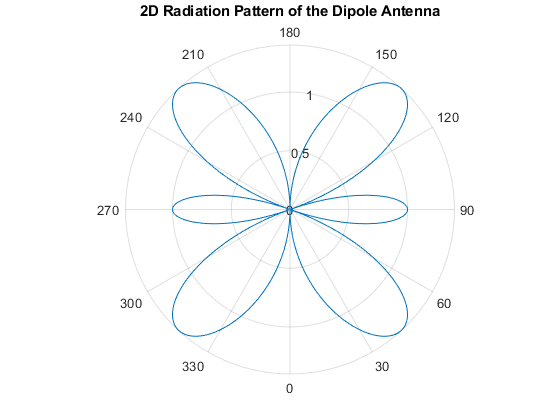
\includegraphics[width=0.49\linewidth]{report/images/linear_antenna_2D.png}
         \hfill
         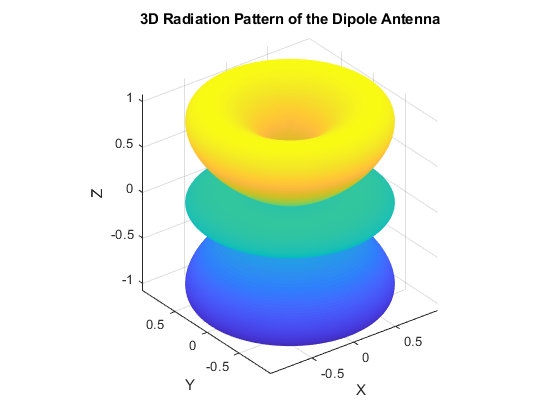
\includegraphics[width=0.49\linewidth]{report/images/linear_antenna_3D.png}
         \caption{Linear Antenna Radiation for $ {l} = {\frac{3}{2}}{\lambda} $}
         \label{fig:Linear Antenna Radiation 3/2}
\end{figure}

\noindent
\textbf{Example:} $ {l} = {2}{\lambda} $
\newline
Similarly, for a dipole length of $ {2}{\lambda} $, the user input is as follows:
\begin{lstlisting}[style=commandstyle,caption=Command line output]]
>> Enter the dipole length as a fraction of the wavelength (e.g., 0.5 for half-wave dipole): 2
\end{lstlisting}

The corresponding radiation patterns are displayed in Figure \ref{fig:Linear Antenna Radiation 2}.
\begin{figure}[H]
    \centering
         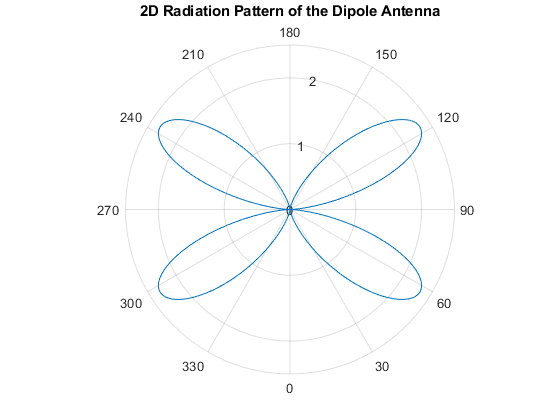
\includegraphics[width=0.49\linewidth]{report/images/linear_antenna_2D_2.png}
         \hfill
         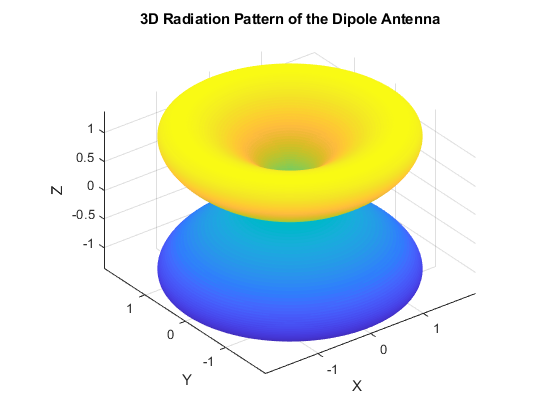
\includegraphics[width=0.49\linewidth]{report/images/linear_antenna_3D_2.png}
         \caption{Linear Antenna Radiation for $ {l} = {2}{\lambda} $}
         \label{fig:Linear Antenna Radiation 2}
\end{figure}

\noindent
The 2-D polar plot demonstrates the radiation pattern of a dipole antenna, highlighting its nulls along the dipole axis. The 3-D visualization shows rotational symmetry around the dipole axis, further confirming the theoretical characteristics of dipole antennas.

%********************************%
%*********SUB-SECTION 2**********%
%********************************%
\subsection{Uniform Linear Antenna Array (ULA)} \label{sec:ula}
\lstinputlisting[style=matlab, caption=MATLAB code, linerange={16-64}]{"../ula.m"}

For a uniform linear array, the array factor $ {AF} $ is expressed as:
\[ {{AF} = {\frac{\sin{\left({{N}{\frac{\psi}{2}}}\right)}}{{N}{\sin{\left({\frac{\psi}{2}}\right)}}}}} \quad\mbox{,} {{\psi} = {{\alpha} + {2}{\pi}{d}{\cos{\left({\gamma}\right)}}}} \]

\noindent
Where:
\begin{itemize}
    \item $ {N} $ is the number of elements in the array,
    \item $ {d} $ is the element spacing as a fraction of the wavelength $ {\lambda} $,
    \item $ {\alpha} $ is the progressive phase shift,
    \item $ {\gamma} $ is the azimuth angle.
\end{itemize}

\noindent
The MATLAB code calculates $ {\psi} $ and the corresponding array factor $ {AF} $ based on user-defined inputs for $ {N} $, $ {d} $, and $ {\alpha} $. The results are visualized in multiple formats:
\begin{itemize}
    \item A 2-D line plot of $ {AF} $ as a function of the azimuth angle $ {\gamma} $,
    \item A 2-D polar plot, and
    \item A 3-D visualization of the radiation pattern.
\end{itemize}

\noindent
\textbf{Example:} $ {d} = {\frac{4}{7}}{\lambda} $, $ {N} = {7} $, $ {\alpha} = -{\frac{4}{7}}{\pi} $.
\newline
The following input demonstrates the configuration:
\begin{lstlisting}[style=commandstyle,caption=Command line output]]
>> Enter the element spacing as a fraction of the wavelength (e.g., 0.5 for half-wavelength): 4/7
   Enter the number of elements in the array: 7
   Enter the progressive phase shift (in radians): -4*pi/7
\end{lstlisting}

The corresponding radiation patterns are depicted in Figure \ref{fig:ula 1}.
\begin{figure}[H]
    \centering
         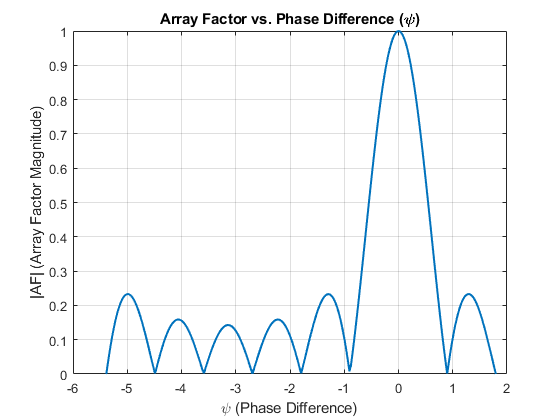
\includegraphics[width=0.49\linewidth]{report/images/ula_2D_1.png}
         \hfill
         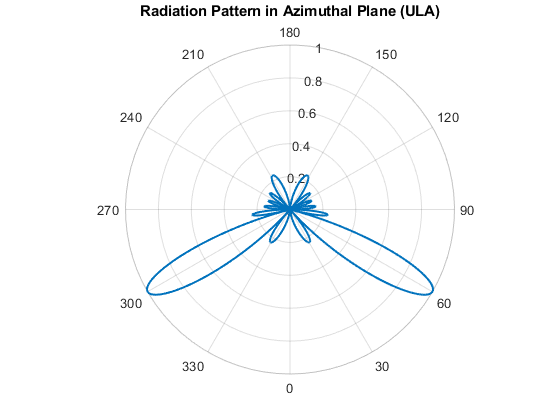
\includegraphics[width=0.49\linewidth]{report/images/ula_2D_rad_1.png}
         \hfill

         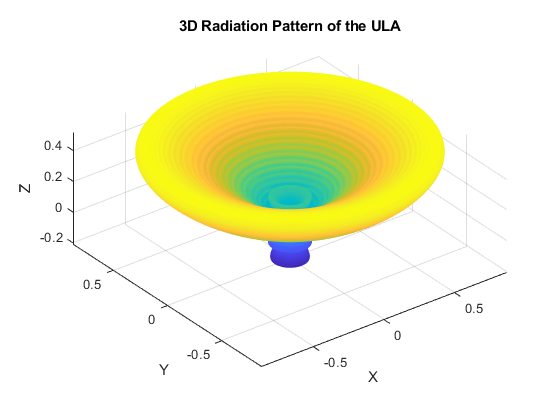
\includegraphics[width=0.49\linewidth]{report/images/ula_3D_1.png}
         \caption{Linear Antenna Radiation for $ {d} = {\frac{4}{7}}{\lambda} $, $ {N} = {7} $, $ {\alpha} = -{\frac{4}{7}}{\pi} $}
         \label{fig:ula 1}
\end{figure}

\noindent
\textbf{Example:} $ {d} = {\frac{5}{12}}{\lambda} $, $ {N} = {6} $, $ {\alpha} = -{\frac{5}{6}}{\pi} $.
\newline
For this configuration, the user input is as follows:
\begin{lstlisting}[style=commandstyle,caption=Command line output]]
>> Enter the element spacing as a fraction of the wavelength (e.g., 0.5 for half-wavelength): 5/12
   Enter the number of elements in the array: 6
   Enter the progressive phase shift (in radians): -5*pi/6
\end{lstlisting}

The resulting radiation patterns are presented in Figure \ref{fig:ula 2}.
\begin{figure}[H]
    \centering
         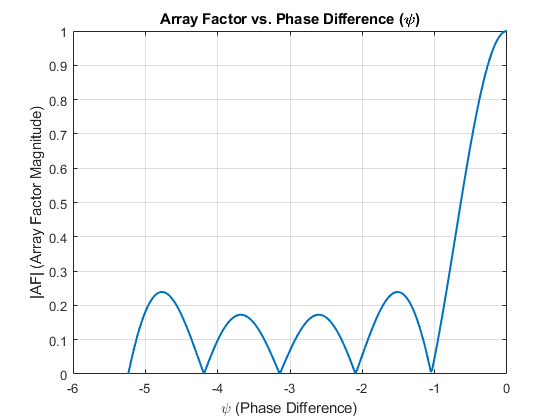
\includegraphics[width=0.49\linewidth]{report/images/ula_2D_2.png}
         \hfill
         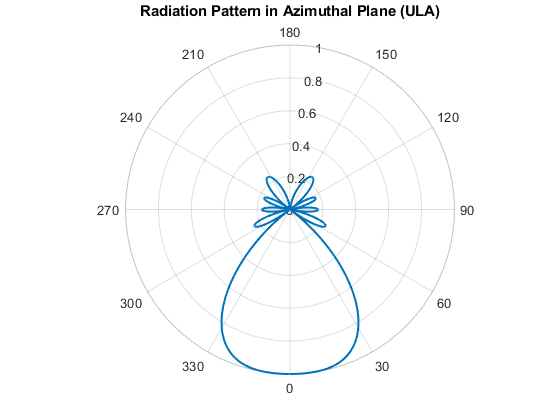
\includegraphics[width=0.49\linewidth]{report/images/ula_2D_rad_2.png}
         \hfill

         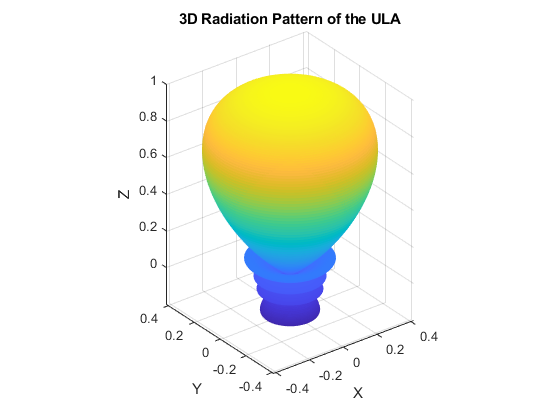
\includegraphics[width=0.49\linewidth]{report/images/ula_3D_2.png}
         \caption{Linear Antenna Radiation for $ {d} = {\frac{5}{12}}{\lambda} $, $ {N} = {6} $, $ {\alpha} = -{\frac{5}{6}}{\pi} $}
         \label{fig:ula 2}
\end{figure}

The 2-D line plots demonstrate the characteristic lobes and nulls of a uniform linear array. The polar plots reveal the directional nature of the array factor, showing maximum radiation in the direction influenced by the phase shift and element spacing. The 3-D visualizations provide a comprehensive view of the array's radiation pattern, emphasizing the symmetry and directivity achieved through specific configurations.
\newline
\noindent
As the element spacing or phase shift changes, the main lobe direction and side lobe levels adjust accordingly, which aligns with theoretical predictions of uniform linear arrays.

%********************************%
%*********SUB-SECTION 3**********%
%********************************%
\subsection{Non-Uniform Linear Antenna Arrays} \label{sec:non-uniform linear array}
\subsubsection{Binomial Array} \label{sec:binomial array}
\lstinputlisting[style=matlab, caption=MATLAB code, linerange={17-63}]{"../binomial_array.m"}

For binomial arrays, the feeding amplitudes follow the coefficients of the binomial expansion to suppress sidelobes. The array factor $ {AF} $ is expressed as:
\[ {{AF} = {\left| \cos ^ {\left( {N} - {1} \right)} {\left( u \right)} \right|}} \quad\mbox{,} {{u} = {\frac{{\alpha} + {2}{\pi}{d}{\cos{\left({\theta}\right)}}}{2}}} \]

\noindent
Where:
\begin{itemize}
    \item $ {N} $ is the number of elements in the array,
    \item $ {d} $ is the element spacing as a fraction of the wavelength $ {\lambda} $,
    \item $ {\alpha} $ is the progressive phase shift,
    \item $ {\theta} $ is the azimuth angle.
\end{itemize}

\noindent
The MATLAB code calculates $ {u} $ and the corresponding array factor $ {AF} $ based on user-defined inputs for $ {N} $, $ {d} $, and $ {\alpha} $. The results are visualized in multiple formats:
\begin{itemize}
    \item A 2-D line plot of $ {AF} $ as a function of the azimuth angle $ {\theta} $,
    \item A 2-D polar plot, and
    \item A 3-D visualization of the radiation pattern.
\end{itemize}

\noindent
\textbf{Example:} $ {d} = {\frac{3}{4}}{\lambda} $, $ {N} = {8} $, $ {\alpha} = {0} $.
\newline
The following input demonstrates the configuration:
\begin{lstlisting}[style=commandstyle,caption=Command line output]]
>> Enter the element spacing as a fraction of the wavelength (e.g., 0.5 for half-wavelength): 3/4
   Enter the number of elements in the array: 8
   Enter the progressive phase shift (in radians): 0
\end{lstlisting}

The corresponding radiation patterns are depicted in Figure \ref{fig:binomial 1}.
\begin{figure}[H]
    \centering
         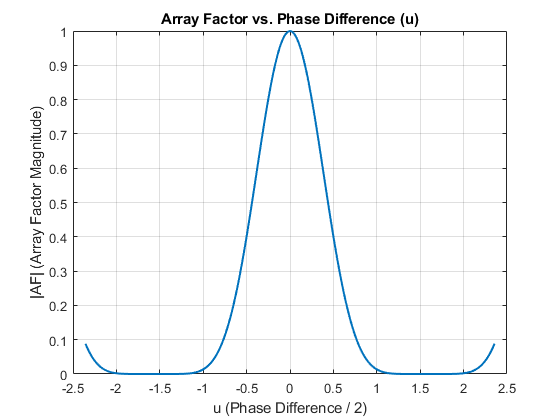
\includegraphics[width=0.49\linewidth]{report/images/binomial_2D_1.png}
         \hfill
         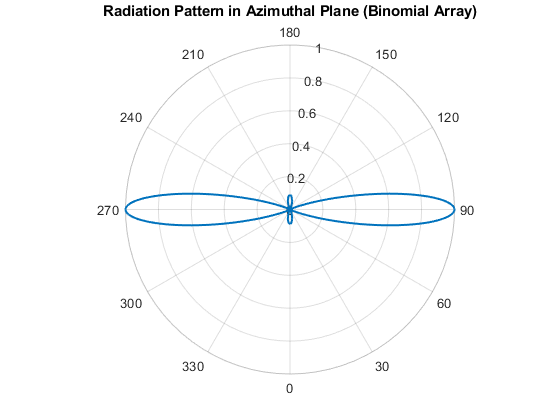
\includegraphics[width=0.49\linewidth]{report/images/binomial_2D_rad_1.png}
         \hfill

         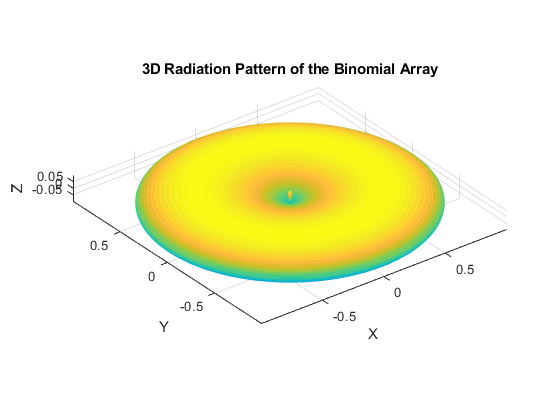
\includegraphics[width=0.49\linewidth]{report/images/binomial_3D_1.png}
         \caption{Binomial Antenna Array Radiation for $ {d} = {\frac{3}{4}}{\lambda} $, $ {N} = {8} $, $ {\alpha} = {0} $}
         \label{fig:binomial 1}
\end{figure}

\noindent
\textbf{Example:} $ {d} = {\frac{1}{4}}{\lambda} $, $ {N} = {8} $, $ {\alpha} = {0} $.
\newline
For this configuration, the user input is as follows:
\begin{lstlisting}[style=commandstyle,caption=Command line output]]
>> Enter the element spacing as a fraction of the wavelength (e.g., 0.5 for half-wavelength): 1/4
   Enter the number of elements in the array: 8
   Enter the progressive phase shift (in radians): 0
\end{lstlisting}

The resulting radiation patterns are presented in Figure \ref{fig:binomial 2}.
\begin{figure}[H]
    \centering
         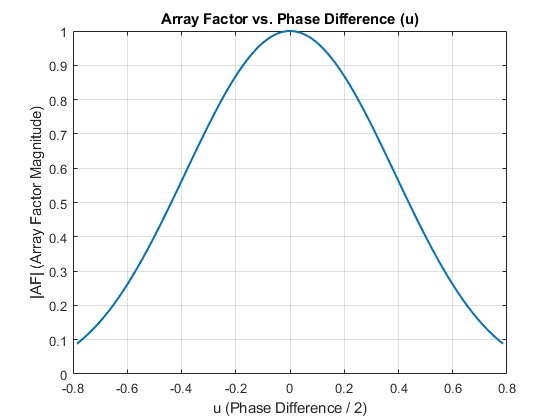
\includegraphics[width=0.49\linewidth]{report/images/binomial_2D_2.png}
         \hfill
         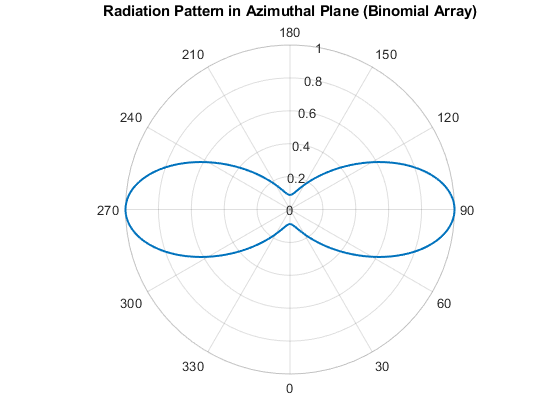
\includegraphics[width=0.49\linewidth]{report/images/binomial_2D_rad_2.png}
         \hfill

         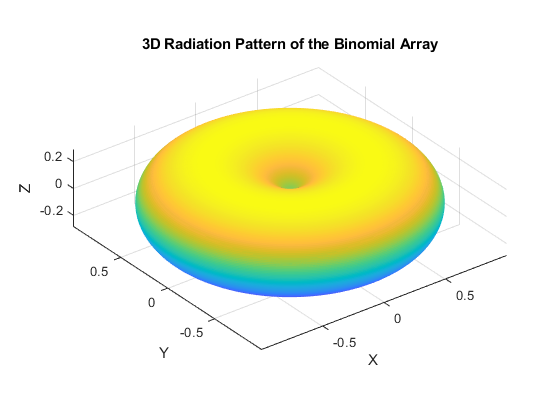
\includegraphics[width=0.49\linewidth]{report/images/binomial_3D_2.png}
         \caption{Linear Antenna Radiation for $ {d} = {\frac{1}{4}}{\lambda} $, $ {N} = {8} $, $ {\alpha} = {0} $}
         \label{fig:binomial 2}
\end{figure}

The binomial array achieves a significant suppression of sidelobes, as observed in both examples. This behavior is consistent with theoretical predictions.
\newline
\noindent
The 3-D visualizations further demonstrate the symmetric nature of the radiation pattern and the absence of significant sidelobes, validating the effectiveness of the binomial feeding approach.

\subsubsection{Dolph-Tschebyscheff Array} \label{sec:dolph-tscheyscheff array}
\lstinputlisting[style=matlab, caption=tshebyscheff function, linerange={1,16-22,25-26}]{"../tshebyscheff.m"}
\lstinputlisting[style=matlab, caption=MATLAB code, linerange={17-67}]{"../dolph_tshebyscheff.m"}

The Dolph-Tschebyscheff array optimizes the trade-off between beamwidth and sidelobe level by using feeding amplitudes determined by Tschebyscheff polynomials. The Tschebyscheff polynomial $ {{T}_{m}}{\left({z}\right)} $ is defined recursively as:
\[ {{{{T}_{0}}{\left({z}\right)}} = {1}} \quad\mbox{,} {{{{T}_{1}}{\left({z}\right)}} = {z}} \quad\mbox{,} {{{{T}_{m}}{\left({z}\right)}} = {{2}{z}{{T}_{{m}-{1}}}{\left({z}\right)}} - {{T}_{{m}-{2}}}{\left({z}\right)}} \]

\noindent
The array factor $ {AF} $ is given by:
\[ {AF} = \left| {{T}_{m}}{\left({{z}_{0} \cdot {\cos{\left({u}\right)}}}\right)} \right| \]

\noindent
Where $ {{Z}_{0}} $ is determined by:
\[ {{z}_{0}} = \cosh{{\frac{1}{m}} \cdot \cosh^{-1}{\left({R}_{0}\right)}} \]
and $ {{R}_{0}} $ is the mainlobe-to-sidelobe level ratio.

\noindent
The MATLAB code calculates the array factor $ {AF} $ based on user-defined inputs for $ {N} $, $ {d} $, $ {\alpha} $, and $ {{R}_{0}} $. The results are visualized in multiple formats:
\begin{itemize}
    \item A 2-D line plot of $ {AF} $ as a function of the azimuth angle $ {\theta} $,
    \item A 2-D polar plot, and
    \item A 3-D visualization of the radiation pattern.
\end{itemize}

\noindent
\textbf{Example:} $ {d} = {\frac{1}{2}}{\lambda} $, $ {N} = {6} $, $ {\alpha} = -{\pi} $, $ {{R}_{0}} = {10} $.
\newline
The following input demonstrates the configuration:
\begin{lstlisting}[style=commandstyle,caption=Command line output]]
>> Enter the element spacing as a fraction of the wavelength (e.g., 0.5 for half-wavelength): 1/2
   Enter the number of elements in the array: 6
   Enter the progressive phase shift (in radians): -pi
   mainlobe to sidelobe level R_o: 10
\end{lstlisting}

The corresponding radiation patterns are depicted in Figure \ref{fig:dolph_tshebyscheff 1}.
\begin{figure}[H]
    \centering
         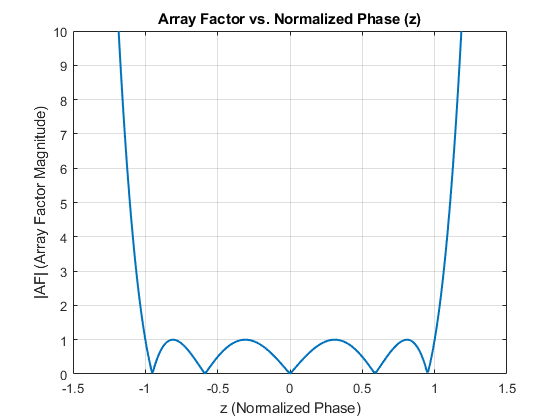
\includegraphics[width=0.49\linewidth]{report/images/dolph_tshebyscheff_2D.png}
         \hfill
         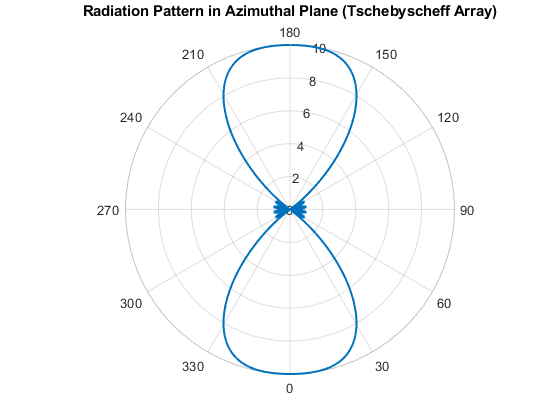
\includegraphics[width=0.49\linewidth]{report/images/dolph_tshebyscheff_rad_2D.png}
         \hfill

         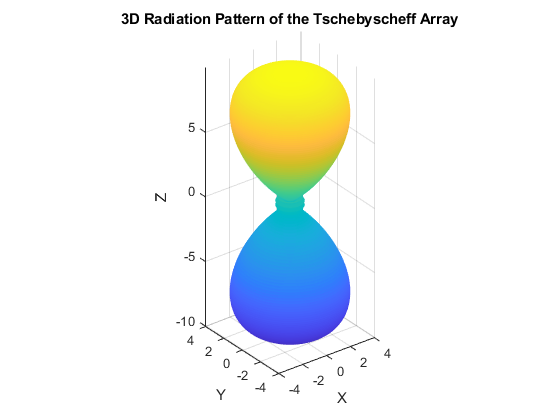
\includegraphics[width=0.49\linewidth]{report/images/dolph_tshebyscheff_3D.png}
         \caption{Dolph-Tschebyscheff Antenna Array Radiation for $ {d} = {\frac{1}{2}}{\lambda} $, $ {N} = {6} $, $ {\alpha} = -{\pi} $, $ {{R}_{0}} = {10} $}
         \label{fig:dolph_tshebyscheff 1}
\end{figure}
The Dolph-Tschebyscheff array produces a highly optimized radiation pattern characterized by:
\begin{itemize}
    \item A narrower mainlobe, providing better directivity,
    \item Well-controlled sidelobes with an amplitude ratio determined by $ {{R}_{0}} $.
\end{itemize}



%********************************%
%***********SECTION 3************%
%********************************%
\section{Conclusion}
This lab investigated various antenna array configurations and their radiation patterns, with a focus on linear antennas, Uniform Linear Arrays (ULA), binomial arrays, and Dolph-Tschebyscheff arrays. Each antenna type was analyzed and simulated using MATLAB, demonstrating the impact of key parameters such as element spacing, number of elements, and phase shifts on the radiation characteristics.
\begin{enumerate}
    \item \textbf{Linear Antenna:} The analysis of a simple dipole antenna demonstrated how the antenna's length relative to the wavelength influences its radiation pattern. The dipole showed characteristic nulls along its axis, consistent with theoretical predictions. The results reinforced the understanding of radiation intensity distribution based on antenna dimensions.
    \item \textbf{Uniform Linear Array (ULA):} For the ULA, the significant impact of the array factor $ {AF} $ on radiation characteristics was observed. By varying the number of elements, element spacing, and phase shift, it was shown how the ULA can direct the radiation pattern and influence the formation of main lobes and sidelobes. These results highlight the role of the array's configuration in optimizing directivity and beamforming capabilities.
    \item \textbf{Binomial Array:} The binomial array, designed to suppress sidelobes by following the binomial amplitude distribution, demonstrated superior sidelobe reduction compared to standard arrays. The simulation results confirmed that binomial arrays focus more energy in the main lobe while reducing undesired radiation in other directions, which is particularly useful for applications requiring high beamforming efficiency.
    \item \textbf{Dolph-Tschebyscheff Array:} The Dolph-Tschebyscheff array was effective in minimizing sidelobes while optimizing the mainlobe width using Tschebyscheff polynomials. By adjusting the mainlobe-to-sidelobe ratio $ {{R}_{0}} $, it was shown how tight control over sidelobe levels can be achieved, which is critical in applications where interference suppression and precision are essential.
\end{enumerate}

\noindent
In conclusion, the versatility of antenna arrays in shaping radiation patterns for specific applications was demonstrated. The simulations using MATLAB provided valuable insights into the effects of design parameters on antenna performance, allowing for the fine-tuning of radiation patterns to achieve optimal characteristics such as directivity, sidelobe suppression, and beamforming. These findings are crucial for the design and optimization of passive antenna systems in various communication, radar, and other electromagnetic applications.


\end{document}